\documentclass[tikz,border=10pt]{standalone}
\usepackage{tikz}
\usetikzlibrary{positioning, calc}

\begin{document}

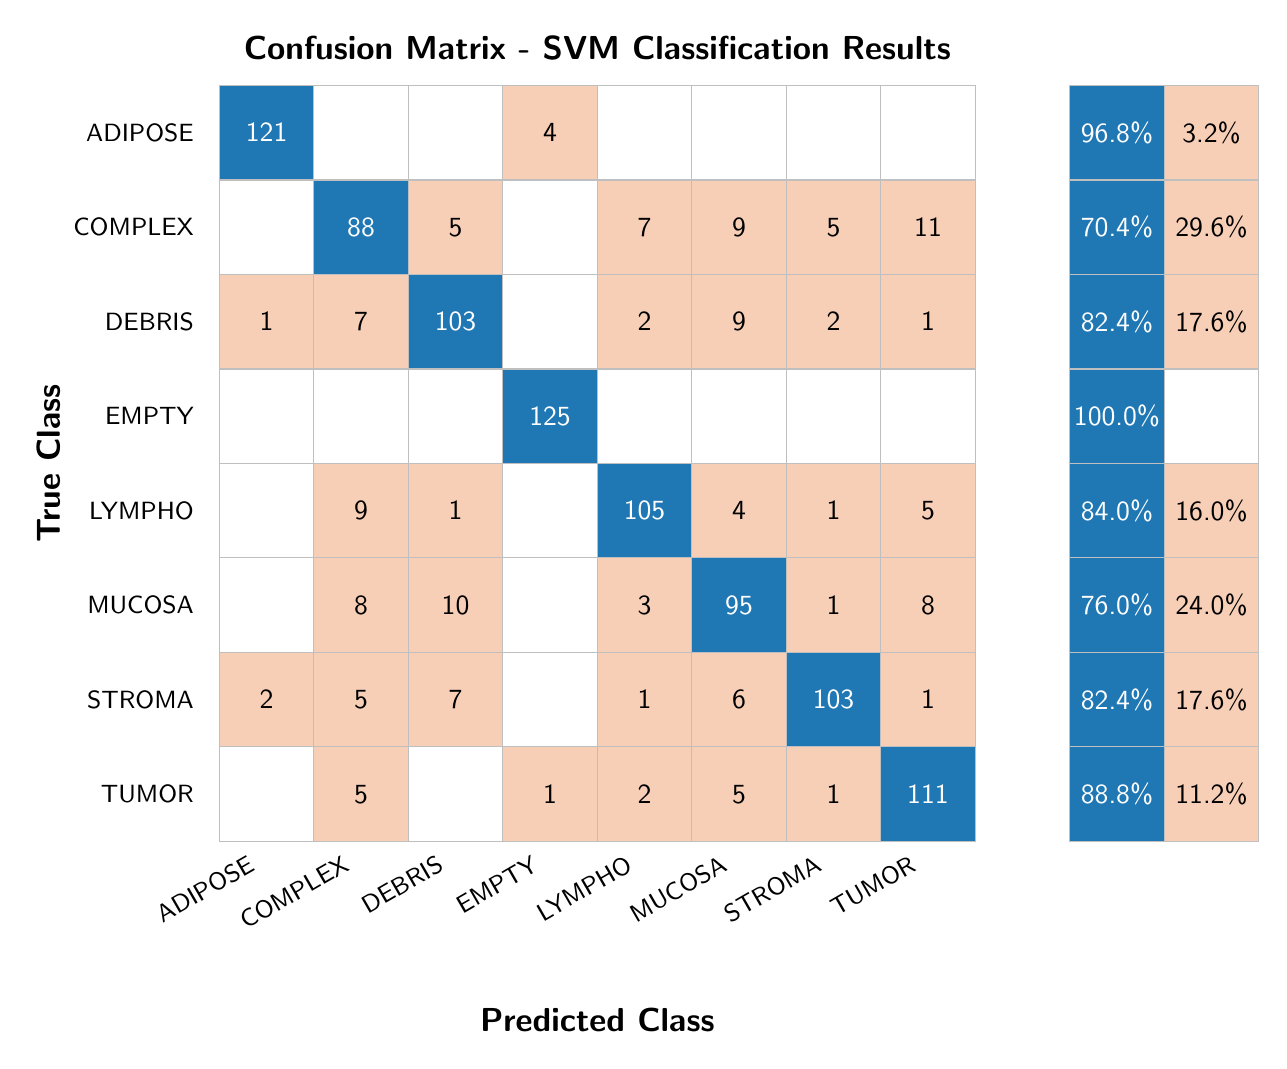
\begin{tikzpicture}[
    cell/.style={rectangle, draw=gray!50, minimum width=1.2cm, minimum height=1.2cm, inner sep=0pt, anchor=center, font=\sffamily},
    bluecell/.style={cell, fill=myblue, text=white},
    orangecell/.style={cell, fill=myorange, text=black},
    label text/.style={font=\sffamily\small, align=right},
    axis label/.style={font=\sffamily\large}
]

% Define colors extracted from image
\definecolor{myblue}{RGB}{31,119,180}
\definecolor{myorange}{RGB}{247,206,182}

% --- Main Confusion Matrix ---
% Draw grid and empty cells first
\foreach \y in {0,...,7} {
    \foreach \x in {0,...,7} {
        \node[cell] (c-\y-\x) at (\x*1.2, -\y*1.2) {};
    }
}

% Fill Diagonal (Blue)
\node[bluecell] at (0*1.2, -0*1.2) {121};
\node[bluecell] at (1*1.2, -1*1.2) {88};
\node[bluecell] at (2*1.2, -2*1.2) {103};
\node[bluecell] at (3*1.2, -3*1.2) {125};
\node[bluecell] at (4*1.2, -4*1.2) {105};
\node[bluecell] at (5*1.2, -5*1.2) {95};
\node[bluecell] at (6*1.2, -6*1.2) {103};
\node[bluecell] at (7*1.2, -7*1.2) {111};

% Fill Off-Diagonal (Orange)
% Row 0
\node[orangecell] at (3*1.2, -0*1.2) {4};
% Row 1
\node[orangecell] at (2*1.2, -1*1.2) {5};
\node[orangecell] at (4*1.2, -1*1.2) {7};
\node[orangecell] at (5*1.2, -1*1.2) {9};
\node[orangecell] at (6*1.2, -1*1.2) {5};
\node[orangecell] at (7*1.2, -1*1.2) {11};
% Row 2
\node[orangecell] at (0*1.2, -2*1.2) {1};
\node[orangecell] at (1*1.2, -2*1.2) {7};
\node[orangecell] at (4*1.2, -2*1.2) {2};
\node[orangecell] at (5*1.2, -2*1.2) {9};
\node[orangecell] at (6*1.2, -2*1.2) {2};
\node[orangecell] at (7*1.2, -2*1.2) {1};
% Row 3 (Empty off-diagonals)
% Row 4
\node[orangecell] at (1*1.2, -4*1.2) {9};
\node[orangecell] at (2*1.2, -4*1.2) {1};
\node[orangecell] at (5*1.2, -4*1.2) {4};
\node[orangecell] at (6*1.2, -4*1.2) {1};
\node[orangecell] at (7*1.2, -4*1.2) {5};
% Row 5
\node[orangecell] at (1*1.2, -5*1.2) {8};
\node[orangecell] at (2*1.2, -5*1.2) {10};
\node[orangecell] at (4*1.2, -5*1.2) {3};
\node[orangecell] at (6*1.2, -5*1.2) {1};
\node[orangecell] at (7*1.2, -5*1.2) {8};
% Row 6
\node[orangecell] at (0*1.2, -6*1.2) {2};
\node[orangecell] at (1*1.2, -6*1.2) {5};
\node[orangecell] at (2*1.2, -6*1.2) {7};
\node[orangecell] at (4*1.2, -6*1.2) {1};
\node[orangecell] at (5*1.2, -6*1.2) {6};
\node[orangecell] at (7*1.2, -6*1.2) {1};
% Row 7
\node[orangecell] at (1*1.2, -7*1.2) {5};
\node[orangecell] at (3*1.2, -7*1.2) {1};
\node[orangecell] at (4*1.2, -7*1.2) {2};
\node[orangecell] at (5*1.2, -7*1.2) {5};
\node[orangecell] at (6*1.2, -7*1.2) {1};

% --- Right Summary Matrix ---
\def\rightoffset{10.8}
% Column 1 (Blue)
\foreach \y/\val in {0/96.8\%, 1/70.4\%, 2/82.4\%, 3/100.0\%, 4/84.0\%, 5/76.0\%, 6/82.4\%, 7/88.8\%} {
    \node[bluecell] at (\rightoffset, -\y*1.2) {\val};
}
% Column 2 (Orange)
\foreach \y/\val in {0/3.2\%, 1/29.6\%, 2/17.6\%, 4/16.0\%, 5/24.0\%, 6/17.6\%, 7/11.2\%} {
    \node[orangecell] at (\rightoffset+1.2, -\y*1.2) {\val};
}
% Empty cell at (3,1) in right matrix
\node[cell] at (\rightoffset+1.2, -3*1.2) {};

% --- Labels ---

% Class Names
\foreach \y/\name in {0/ADIPOSE, 1/COMPLEX, 2/DEBRIS, 3/EMPTY, 4/LYMPHO, 5/MUCOSA, 6/STROMA, 7/TUMOR} {
    % Y-axis labels (Left of main matrix)
    \node[label text, anchor=east] at (-0.8, -\y*1.2) {\name};
    
    % X-axis labels (Rotated, moved up to just below the main matrix)
    % The bottom of the last cell (row 7) is at y = -7*1.2 - 0.6 = -9.0
    \node[label text, anchor=north east, rotate=30] at (\y*1.2 - 0.2, -9.0) {\name};
}

% Main Title
\node[font=\sffamily\bfseries\large, anchor=south] at (4.2, 0.8) {Confusion Matrix - SVM Classification Results};

% Axis Titles
\node[axis label, rotate=90, anchor=south] at (-2.5, -4.2) {\textbf{True Class}};
\node[axis label, anchor=north] at (4.2, -11.0) {\textbf{Predicted Class}};

\end{tikzpicture}

\end{document}